\section{Structured Independent-Edge Random Network}
\label{sec:ch5:siem}

Next up, we'll cover a statistical model for networks which generalizes the SBM from Section \ref{sec:ch5:sbm} a little differently than the IER network from Section \ref{sec:ch5:ier}. Sometimes in a network, there might particular pairs of nodes which, when those nodes are incident a particular edge, impart a different distribution for that edge. Let's consider an example, which boils back to the example that we gave in Chapter \ref{sec:ch2}. Imagine we have a network, where the $n=100$ nodes are different areas of the brain.  Each of these nodes are either in the left, or the right, side of the brain. An edge exists, or does not exist, if the two areas of the brain tend to be active together while a person iteracts with the world. A particular notion that scientists hypothesis is that, even though the left and right sides of the brain tend to have different functions, the nodes on the left and right sides still might tend to be active together, especially when it is the same region on both sides. 

For instance, even though the motor cortex (responsible for {motion} and {conscious movement}) in the left hemisphere has different jobs from the motor cortex in the right hemisphere, the jobs provided by each hemisphere tend to work in tandem, with the right motor cortex providing movement for the left side of the body, and the left motor cortex provides movement for the right side of the body. When someone is moving around, a lot of tasks will require them to use both sides of the body in tandem, so even though the two motor cortices are doing different jobs, they still tend to be active together. This pattern, known as \textit{bilateral homotopy}, tends to trickle down to many other areas in the brain as well. Let's turn this into a question: do bilateral node pairs have higher connectivity than non-bilateral node pairs?

So, how do you actually study this property? As we have learned in this chapter so far, we want statistical models which capture what we understand about the system. What you understand is that, perhaps, the edges between pairs of nodes which are bilaterally symmetric tend to be more likely than the edges between pairs of nodes which are not bilaterally symmetric. Based on what we know so far, you could easily reflect this using the $IER_n(P)$ random network: Allow every pair of nodes in the network to have their own edge probability, and then the system works out.

If we wanted to use our data (one network, with an adjacency matrix $A$) to describe this system, we are at quite a loss, unfortunately. On one hand, our network model is much simpler than a model which ascribes probabilities to every possible network configuration for an $n$ node simple network (of which there are $2^{\binom n 2}$ of them, as-per Remark \ref{box:ch5:whyuse}). On the other, this model still has $\binom n 2$ parameters (the entries of the probability matrix $P$), one for each individual edge in the network. This is, in a sense, still exactly equivalent to the coin flipping problem from Remark \ref{box:ch5:whyuse}: to learn about a probability $p_{ij}$, we have exactly one edge $a_{ij}$. Learning about $p_{ij}$ from a single edge $a_{ij}$ is exactly as pointless as trying to learn about the probability a coin lands on heads from the outcome of a single coin toss.

Instead, we will conceptualize this problem a little bit differently using the Structured Independent Edge Model (SIEM).
\subsection{The Structured Independent Edge Model is parametrized by a Cluster-Assignment Matrix and a probability vector}
\subsubsection{The Cluster-Assignment Matrix}

The cluster assignment matrix $D$ is an $n \times n$ matrix which assigns potential edges in the random network to clusters. What do we mean by this?

Remember that the adjacency matrix $\mathbf A$ for a random network is {also} an $n \times n$ matrix, where each entry $\mathbf a_{ij}$ is a random variable which takes the value $0$ or the value $1$ with a particular probability. The cluster assignment matrix takes each of these $n^2$ random variables, and uses a parameter $v_{ij}$ to indicate which of $K$ possible clusters this edge is part of. In the brain example above, for instance, we could take $v_{ij} = 1$ when the nodes $i$ and $j$ are bilateral pairs, and $v_{ij} = 2$ when the nodes $i$ and $j$ are not bilateral pairs. For simple networks, we'll also add the restriction that $v_{ij} = v_{ji}$ for all node pairs $i$ and $j$, and we'll leave $z_{ii}$ to be unassigned (a value of \texttt{NA}) since simple networks are loopless.

\subsubsection{The Probability vector}

The second parameter for the SIEM is a probability vector, $\vec p$. If there are $L$ edge clusters in the SIEM, then $\vec p$ is a length-$L$ vector. Each entry $p_l$ indicates the probablity of an edge in the $l^{th}$ cluster existing in the network. For example, $p_1$ indicates the probability of an edge in the first edge cluster, $p_2$ indicates the probability of an edge in the second edge cluster, so on and so-forth. In the brain example, for instance, $p_1$ would represent the probability of an edge between a pair of nodes that represent the same brain area in opposite hemispheres (bilateral pairs), and $p_2$ would represent the probability of an edge between a pair of nodes that are not bilateral pairs.

\subsection{Conceptualizing the SIEM}

Like usual, we will formulate the SIEM using our old coin flip example. We begin by obtaining $L$ coins, where the $k^{th}$ coin has a chance of landing on heads of $p_k$, and a chance of landing on tails of $1 - p_k$. For each entry $\mathbf a_{ij}$, we identify the corresponding cluster $v_{ij}$ that this edge is in. Remember that $v_{ij}$ takes one of $L$ possible values. We flip the $v_{ij}$ coin, and if it lands on heads (with probability $p_{v_{ij}}$), the edge exists, and if it lands on tails (with probability $1 - p_{v_{ij}}$) the edge does not exist.

If $\mathbf A$ is an SIEM random network with $n$ nodes, the cluster assignment matrix $D$, and the probability vector $\vec p$, we say that $\mathbf A$ is an $SIEM_n(D, \vec p)$ random network.

\subsubsection{How do we simulate samples from an $SIEM_n(D, \vec p)$ random network?}

The procedure in Algorithm \ref{alg:ch5:siem} will produce for us a network $A$, which has nodes and edges, where the underlying random network $\mathbf A$ is an $SIEM_n(D, \vec p)$ random network.

\begin{algorithm}[h]\caption{Simulating a sample from an $SIEM_n(D, \vec p)$ random network}
\label{alg:ch5:siem}
\SetAlgoLined
\KwData{$n$ a number of nodes\newline $D$ a matrix which assigns one of $L$ edge-clusters to each of the $n^2$ edges \newline $\vec p$ a $L$-dimensional probability vector for each edge-cluster}
\KwResult{The adjacency matrix of a sample from the random network.}

For each of the $L$ clusters, obtain $L$ total weighted coins, where the $k^{th}$ coin lands on heads with probability $p_k$ and tails with probability $1 - p_k$.

\For{$i$ in $1$:$n$}{
    \For{$j > i$}{
        Flip the $v_{ij}$ coin, and if it lands on heads, the corresponding entry in the adjacency matrix $a_{ij}$ is $1$. If it lands on tails, the coresponding entry in the adjacency matrix $a_{ij}$ is $0$. 

        Let $a_{ji}= a_{ij}$.
    }
}

\Return{$A$}
\end{algorithm}

Let's turn back to our network example we looked at. The first fifty nodes will be the areas in the left hemisphere of the brain, and the second fifty nodes will be the areas of the right hemisphere of the brain. The nodes will be sequentially ordered, so that the first node of the left is the first node of the right, so on and so forth, for all $50$ pairs of nodes. Further, programmatically, it is much easier to encode \texttt{NA} as $0$, so we fill the diagonal with $0$s. Since the network we are generating is simply, these entries won't matter for our sample that we generate anyways. We can generate a cluster assignment matrix like this:

\begin{lstlisting}[style=python]
import numpy as np

n = 100
D = np.ones((n, n))
for i in range(0, int(n/2)):
    D[int(i + n/2), i] = 2
    D[i, int(i + n/2)] = 2
np.fill_diagonal(D, 0)
\end{lstlisting}

We'll also visualize the cluster assignment matrix along with the hemisphere of each brain node:

\begin{lstlisting}[style=python]
from graphbook_code import heatmap

labels = ["L" for i in range(0, int(n/2))] + ["R" for i in range(0, int(n/2))]
heatmap(D.astype(int), title="Cluster assignment matrix", 
        inner_hier_labels=labels)
\end{lstlisting}

The cluster assignment matrix is shown in Figure \ref{fig:ch5:siem}(A). As we can see, there are several ``bands'' going across this matrix. The bands are the stripes moving diagonally across the cluster assignment matrix. The white band is the diagonal entries. Since the networks we are dealing with are simple, they are undirected, so we do not need to worry about the diagonal entries.

In the off-diagonal entries, we can see another band. This band consists of the bilateral pairs of nodes; remember that the first node of the left hemisphere was the same functional area of the brain, but just in the other hemisphere. Hence, these edges are "assigned" to cluster $2$. Remember that the nodes are organized such that the first $\frac{n}{2}$ nodes are area $1$ for hemisphere $L$, so on and so forth for all areas of the left hemisphere. Next, the remaining $\frac{n}{2}$ nodes corresponding area $1$ for hemisphere $R$, so on and so forth for all of the areas of the right hemisphere. Therefore, this pattern will manifest as an ``offset'' band, where the ``offset'' amount of offset is simply the number of nodes between area $u$ in hemisphere $L$ and area $u$ in hemisphere $R$ (which is $\frac{n}{2}$ nodes in total). 

The remaining off-diagonal entries are not bilateral pairs of nodes. These entries are assigned to cluster $1$.
 

Next, we need a probability vector for the two clusters of off-diagonal entries. We will arbitrarily say that there is a $0.8$ probability that an edge adjoining two bilateral pairs of nodes (cluster $2$) is connected, but a $0.1$ probability that an edge adjoining two non-bilateral pairs of nodes (edge cluster $1$) is connected:

\begin{lstlisting}[style=python]
from graphbook_code import siem

p = [0.1, 0.8]
A = siem(n, p, D)
heatmap(A.astype(int), title="$SIEM_n(D, \\vec p)$ sample", 
        inner_hier_labels=labels)
\end{lstlisting}

The adjacency matrix is plotted in Figure \ref{fig:ch5:siem}(B). Notice that the adjacency matrix reflects the same banding pattern of the cluster assignment matrix. 

\begin{figure}[h]
    \centering
    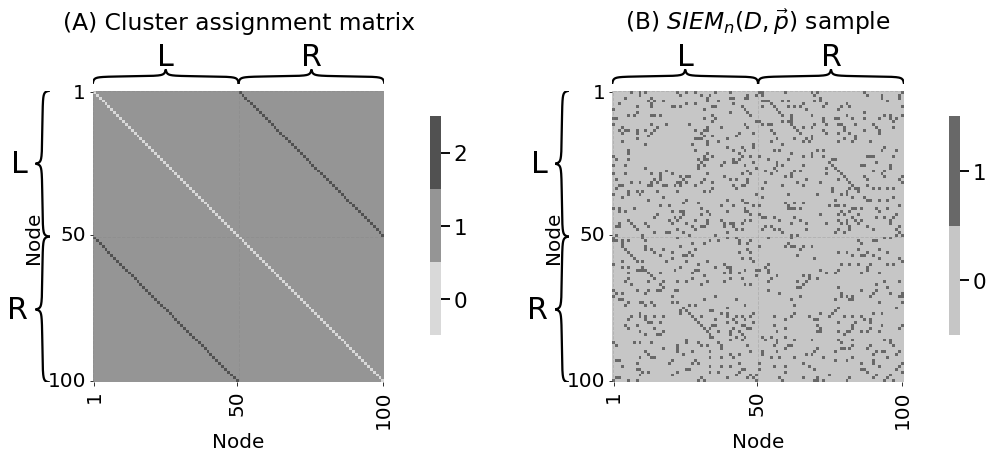
\includegraphics[width=\linewidth]{representations/ch5/Images/siem.png}
    \caption[Visualizing SIEM networks]{\textbf{(A)} the cluster assignment matrix $D$. \textbf{(B)} sample of an adjacency matrix from an $SIEM_n(D, \vec p)$ random network. }
    \label{fig:ch5:siem}
\end{figure}
\subsection{What is the relationship between the $SIEM_n(D, \vec p)$ random network and the $SBM_n(\vec z, B)$ random network?}

If you recall from Section \ref{sec:ch5:ier:ier_generalises}, we spent a lot of effort determining which networks were more complex than other networks. We can do this for the $SIEM_n(D, \vec p)$ random networks, too. 

We are going to demonstrate that every simple $SBM_n(\vec z, B)$ random network with $K < n$ communities can be represented as a simple $SIEM_n(D, \vec p)$ random network with $L < \binom n 2$ communities. The $SIEM_n(D, \vec p)$ with $L < \binom{n + 1}{2}$ is a similar level of complexity to the $SBM_n(\vec z, B)$ with $K < n$, because the block matrix for a $SBM_n(\vec z, B)$ with $K < n$ has less than $\binom{n + 1}{2}$ unique entries.

At an extremely high level, what we do is, for each pair of communities $k$ and $k'$, we define a unique edge-cluster $l$. Next, for each pair of nodes $i$ and $j$, we check which communities they are part of, and then define $v_{ij}$ to be the edge cluster that corresponds to that pair of communities.

Finally, for the probability vector, we just take $p_l$ for a given edge-cluster $l$ to be the entry of $B$ whose indices mapped to edge-cluster $l$. For instance, if communities $k$ and $k'$ mapped to edge-cluster $l$, we take $p_l = b_{kk'}$. The resulting $SIEM_n(D, \vec p)$ random network has the same probability matrix as the $SBM_n(\vec z, B)$ random network, so all SBMs  with $K < n$ are SIEMs with $L < \binom{n + 1}{2}$.

The reverse is not true; the example provided here regarding bilateral brain areas is a counter example that cannot be represented using an $SBM_n(\vec z, B)$ random network with a number of communities $K < n$.

For this reason, the $SIEM_n(D, \vec p)$ with $L < \binom{n+1}{2}$ is more complex than the $SBM_n(\vec z, B)$ with $K < n$.

In later sections such as Section \ref{sec:ch7:testing}, we will develop statistical tools for $SIEM_n(D, \vec p)$ random networks, but it is important to note that they apply equally well to $SBM_n(\vec z, B)$ random networks. The statistical tools afforded to the SIEM will allow you to capture more general questions than just those you could ask with the SBM, in which you can look for differences between pairs of groups of edges, rather than just looking for differences between pairs of groups of nodes, since there can be complicated arrangements of edges which are not easily capturable with the SBM.


\newpage